\documentclass[letterpaper,conference]{IEEEtran}

\usepackage[backend=biber,style=apa,citestyle=apa]{biblatex}
\addbibresource{mendeleybib/tesis.bib}

%Idioma y caracteres del idioma
\usepackage[utf8]{inputenc}
\usepackage[spanish]{babel}


\usepackage{float}
\usepackage{caption}
\usepackage{subcaption}	
\usepackage{stix}        %para el elerdendots para el rango


\usepackage{datetime}	%fecha
\usepackage{mfirstuc}	%mayuscula
\usepackage{lipsum}



\usepackage{listings} %codigos de programas

%Opciones de márgenes
\usepackage[left=3cm,right=3cm,top=2.5cm,bottom=2.5cm]{geometry}

\newdateformat{monthyeardate}{%
\monthname[\THEMONTH ] \THEYEAR}

\usepackage{makeidx}
\usepackage{subfiles}
\usepackage{xcolor}	%colores


\usepackage{lipsum}% http://ctan.org/pkg/lipsum


\newcommand{\tarea}[1]{
{\huge\color{red}{#1}}
}


\newcommand{\tarealista}[1]{
{\Large\color{blue}{#1}}
}
\usepackage{url}
%Paquete para gráficos, por ejemplo colocar imágenes
\usepackage[pdftex]{graphicx}

%Paquete para ecuacioens y/o otros elementos matemáticos
\usepackage{amsmath,amsfonts,amsthm, bm}
\usepackage{mathtools}

\DeclarePairedDelimiter\ceil{\lceil}{\rceil}
\DeclarePairedDelimiter\floor{\lfloor}{\rfloor}

%Paquetes para alinear texto y/o ecuaciones
\usepackage{array}

% Distintas opciones de itemizdo
\usepackage{enumitem}

%Opciones de tabla
\usepackage{multirow}





\begin{document}

\title{Control de recursos en invernadero automatizado mediante un modelo de optimización}

\author{\IEEEauthorblockN{Hans Raddatz García\IEEEauthorrefmark{1},
Samantha Reid Calderón\IEEEauthorrefmark{2} \\Nestor Palominos Gonzalez\IEEEauthorrefmark{3}, Franco Menares\IEEEauthorrefmark{4}}

\IEEEauthorblockA{\IEEEauthorrefmark{1} \footnotesize	 Universidad Andrés Bello. Estudiante. Facultad de Ingeniería. Chile. E-mail: hansraddatzreyking@gmail.com}
\IEEEauthorblockA{\IEEEauthorrefmark{2} \footnotesize	 Universidad Andrés Bello. MSc.,Docente Facultad de Ingeniería. Chile. E-mail: s.reid.cal@gmail.com}
\IEEEauthorblockA{\IEEEauthorrefmark{3} \footnotesize	 Universidad Andrés Bello. Docente. Departamento de ciencias de la ingenieria. Chile. E-mail: nestor.palominos@gmail.com}	
\IEEEauthorblockA{\IEEEauthorrefmark{4} \footnotesize	 Universidad Andrés Bello. Facultad de Ingeniería. Chile. E-mail: Francomenares@gmail.com}
}
\maketitle

% Para colocar el título
\maketitle

%Para ponerle número de página al documento
\thispagestyle{plain}
\pagestyle{plain}

\begin{abstract}
Se aborda el problema de gestión de un invernadero automatizado, el cual aborda desde su confección, gestión y control. En este trabajo se abordan múltiples metodologías, ya que se presenta su confección a través de los sensores a utilizar, el modelo de optimización que busca minimizar costos y un sistema de gestión que permite la integración de estos elementos. La metodología se aplica con los datos reales obtenidos con este invernadero, el cual estará instalado en la Región Metropolitana, Chile. Como resultado, se espera tener un sistema integrado que permita su automatización y gestión de manera continua, el cual proporcione los menores costos de operación con respecto a otros vistos en la literatura.
\end{abstract}

\begin{IEEEkeywords}
	Invernaderos, Modelo de Optimización, Automatización.
\end{IEEEkeywords}

\IEEEpeerreviewmaketitle

\section{INTRODUCCIÓN}

Uno de los grandes problemas que afronta la agricultura es la creciente demanda de alimentos respecto a la disminución de tierra arable \textcite{Specht2014}, además del inminente agotamiento de los recursos hídricos a nivel mundial  \parencite{Baldos2016}. Una forma para combatir estos problemas es mediante invernaderos lo suficientemente flexibles como para ser colocados en cualquier superficie y condiciones, además de ser más eficientes que los cultivos en tierra firme en el uso de recursos como el agua.

Como es importante buscar que la implementación y uso de los invernaderos sea más eficientes que el cultivo tradicional, se utilizarán tecnologías como el SDI (irrigación por goteo en sub-suelo), el cual ha demostrado tener un aprovechamiento del agua de entre el 20\% y el 30\% más que los Sprinklers \parencite{Zaccaria2017}. Otro de los aspectos es la calefacción e iluminación, las cuales no son consideradas para los cultivos tradicionales en tierra y sin techo, a diferencia de los invernaderos en donde la calefacción suele ser el punto más crítico por su alto consumo en temporadas y/o zonas frías \textcite{Dong2018}, por ello la calefacción es uno de los puntos con mayor literatura al respecto donde se rescata el uso de calefacción en el subsuelo como lo plantea \parencite{Kurpaska2000}. El último factor importante que abarca este trabajo es el de la iluminación, el cual solo afecta cuando el invernadero no tiene acceso a luz solar o esta es muy escasa, siendo mencionado en \parencite{VanIersel2017}, donde los requerimientos para la fotosíntesis de las plantas puedes ser asistidos o remplazados completamente con iluminación LED (diodo emisor de luz).

En este documento se presenta una propuesta de invernadero tal que este pueda ser instalado sobre cualquier superficie. Este invernadero utilizará las tecnologías de SDI para la irrigación, calefacción en sub-suelo e iluminación LED asistida, todos controlados por un microcontrolador ESP32 el cual realizará el actuamiento de cada sistema, además de registrar dichos procesos a una base de datos MySQL a través de mensajes en formato JSON en el protocolo MQTT para poder así agregar otras aplicaciones gráficas para una gestión cómoda del invernadero. Además del sistema de gestión se desarrolla un modelo de optimización con Gurobi, el cual busca minimizar el costo operacional para la calefacción e irrigación en el uso de agua y electricidad.



\section{REVISIÓN DE LA LITERATURA}

%Se coloca la revisión de la literatura. Si se quiere citar al autor dentro del documento, ocupar citet, y si se quiere citar luego de una idea, ocupar citetp.

%Posteriormente, se habla de lo que no hay en la literatura, junto con la propuesta del modelo del trabajo.


%hacer mas competitivo el ionvernadero
%It is obvious that future food infrastructure will have to be more productive than today’s food infrastructure, but it will also have to be more sustainable. Sustainable urban food production needs to address all the dimensions of sustainability at the same time. It needs to address envi- ronmental challenges, to tackle and improve social issues, and provide economic welfare.\textcite{Specht2014}

En el futuro la infraestructura para la agronomía tendrá que ser más productiva y sustentable, teniendo foco en mejorar los problemas medio-ambientales y sociales, además de proveer un beneficio económico al mismo tiempo \parencite{Specht2014}.


%mediante automatizacion (tecnologias)

Dentro de las herramientas disponibles para lograr invernaderos más eficientes se destaca el uso de SDI en comparación con el sistema tradicional de Sprinklers, tal como lo demostró el autor \parencite{Of2000}. Esta tecnología no ha tenido tanto impacto como los Sprinklers principalmente por la escasa información accesible para los granjeros y complicaciones que esta puede presentar \parencite{Lamm2012}, a pesar de que la gran mayoría son solucionables como lo demostró \parencite{Yu2010}. 
Otra herramienta que cabe destacar para mejorar la eficiencia de un invernadero es el uso de calefacción en el subsuelo, propuesto por\parencite{Cuce2016}. Dentro de sus propuestas utiliza un modelo de optimización para minimizar la temperatura de los tubos de calefacción. Asimismo, \parencite{Kurpaska2000} determinó que, en gran cantidad de casos, es sustancialmente más eficiente el uso de calefactores en el sub-suelo. 
Otro factor importante es el uso de iluminación asistida, mediante la cual permite sustituir o apoyar a la luz solar que llega a las plantas. Existen las tecnologías de HPS (lámparas de sodio a alta presión) y LED, donde esta última permite la emisión de frecuencias específicas necesarias para fotosíntesis, además de que su emisión puede ser modulada evitando la sobre exposición \parencite{VanIersel2017}.







Mientras que los autores anteriores explicaron cómo utilizar dichas tecnologías, otros optimizaron su uso, tomando como base el trabajo de \parencite{Gijzen1998}, debido a que abarcó sus siete sub-modelos en el funcionamiento de un invernadero. Asimismo, al igual que muchos otros autores más contemporáneos, algunos autores dejaron de lado la optimización para la irrigación, con algunas pocas excepciones en el uso de SDI como lo es \parencite{Kandelous2010}, quien modeló dicha tecnología para obtener el patrón de regadío que esta genera, minimizando el uso de agua. Para el caso de la calefacción existen múltiples propuestas para minimizar su costo, las cuales se pueden dividir según si emplean una heurística o no. Cabe destacar que quienes no hacen uso de esta herramienta suele deberse a que su modelo incluye más variables además de la calefacción, como fue el caso de \parencite{Kiyan2013}, quien buscó un modelo y control automatizado para alternar entre uso de energía solar o combustible fósil para calefaccionar. Los autores que sí utilizaron heurísticas poseyeron bastantes puntos en común respecto a su modelamiento, como lo es el método de utilizar un calefactor para el aire atrapado o el uso de técnicas similares como son el PSO (optimización de enjambre de particulas) \parencite{Hasni2011,Chen2018}, o por CDF (dinámica de fluidos computacional). Estas técnicas se utilizan para modelar la dinámica del aire calefaccionado y, por ende, el movimiento de la temperatura, el cual suele ser de alta complejidad matemática \parencite{Singhal2017}.

Este trabajo propone múltiples metodologías. Primero, se confeccionará un invernadero con el uso de SDI, calefacción de subsuelo e iluminación de asistida. Segundo, se diseñará un modelo de optimización matemática que minimice los costos operaciones. Por último, se elaborará un sistema de gestión para la integración remota del invernadero, el cual podrá tener un control sobre los sistemas anteriormente propuestos. Este trabajo tiene como contribución una propuesta integrada, el cual permita tener un invernadero funcionando y que permita gestionar sus actividades al menor costo.



\section{METODOLOGÍA}


	El invernadero propuesto consta de 3 componentes; el invernadero como estructura física, el modelo de optimización el cual define el comportamiento futuro del invernadero y un sistema de gestión que permita la interacción entre los dos elementos anteriores. La interacción entre los componentes se ejemplifica en la figura \ref{fig:sistemas}, donde se observa que el invernadero proporciona los estados al sistema de gestión, éste se los otorga como parámetros al modelo, dando como resultado una solución y un control al mismo.

		\begin{figure}[ht]
			\centering
				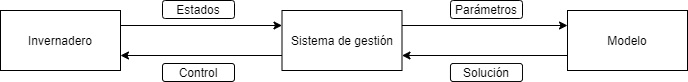
\includegraphics[width=\linewidth]{imagenes/Sistemas.png} 
			\caption{Relación entre sistemas desarrollados}
			\label{fig:sistemas}
		\end{figure}

	\subsection{INVERNADERO}
		El invernadero desarrollado se compone de: estructura física, que alberga y aísla a las plantas; actuadores, tales como bombas, calefactor y luminaria; elementos de medición (sensores) y una caja con la electrónica necesaria para la interacción de los elementos anteriores.
		
		
		\subsubsection{ESTRUCTURA}
			La estructura del invernadero se compone por un armazón de madera, paredes aislantes de termo-paneles de polietileno y en la base una capa de [5cm] de poliestireno expandido. Esta estructura alberga todos los actuadores y sensores. En la Figura \ref{fig:maqueta} se presenta un modelo 3D de como se vera el resultado final.
			\begin{figure}[h]%
				\centering
				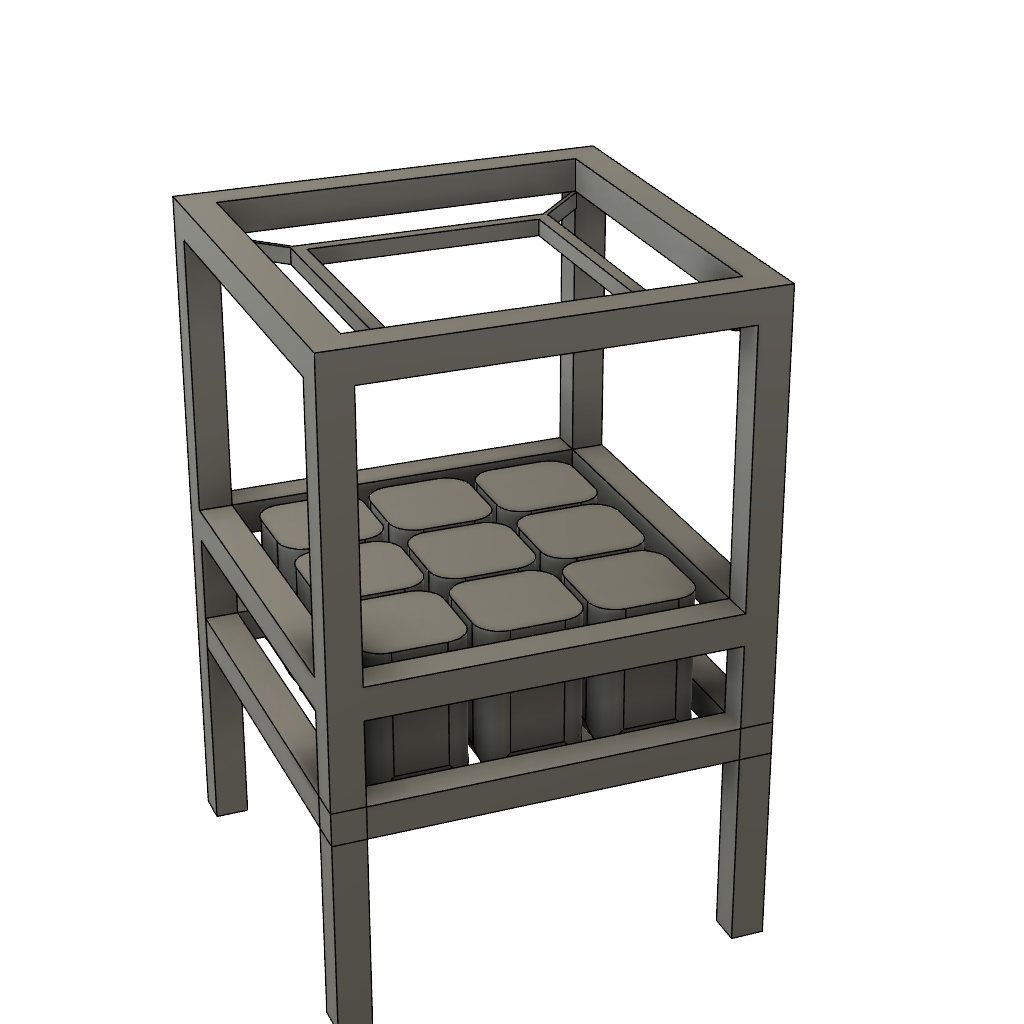
\includegraphics[width=0.35\linewidth]{imagenes/cajon3d.png}%
				\caption{Modelo estructura 3D}
				\label{fig:maqueta}%
			\end{figure}%			

		\subsubsection{CAJA}
		
			al exterior de la estructura estará presente una caja estanca, el cual contiene los mecanismos de control para los actuadores (bombas, iluminación LED y calefactor) ubicados en el invernadero, además de un microcontrolador ESP-32-WROOM y una fuente de poder.

			



		El funcionamiento del invernadero se realiza mediante el control de tres variables en su interior iluminación, temperatura e irrigación. Primero, la iluminación asistida es controlada de forma proporcional según la iluminación resultante de la luminaria LED más la iluminación natural esperada para un tiempo determinado en el día. Después, la irrigación será controlada por la variable de irrigación $BA$ que entrega el modelo desarrollado. Esta permitirá accionar la bomba de irrigación para rellenar una columna de agua, la cual generará una presión de valor conocida sobre el tubo de goteo en el subsuelo. Finalmente esta presión provocará un goteo que humedecerá la tierra de cada contenedor de forma similar. Finalmente, la temperatura será regulada a través del modelo matemático, donde se accionará tanto la bomba de temperatura como el calefactor según la variable de calefaccionar $BT$. El calefactor calienta el agua del módulo principal y la bomba circula esta agua calentada por una tubería de cobre que atraviese a cada submódulo.
				
		
		% el calor se transferirá como se muestra en la Figura \ref{fig:flujo_calor}.
		
	\begin{figure}[h!]
		\centering
		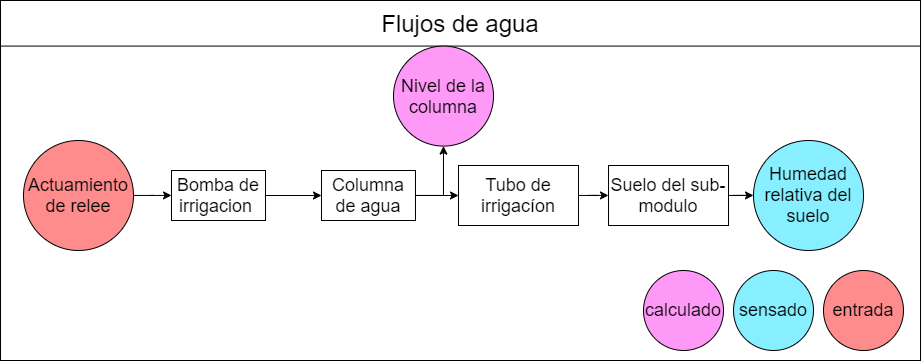
\includegraphics[width=.85\linewidth]{imagenes/flujos de agua.png} 
		\caption{Relación entre sistemas desarrollados}
		\label{fig:flujo_agua}
	\end{figure}						
			
			
%			\begin{figure}[h]
%				\centering
%				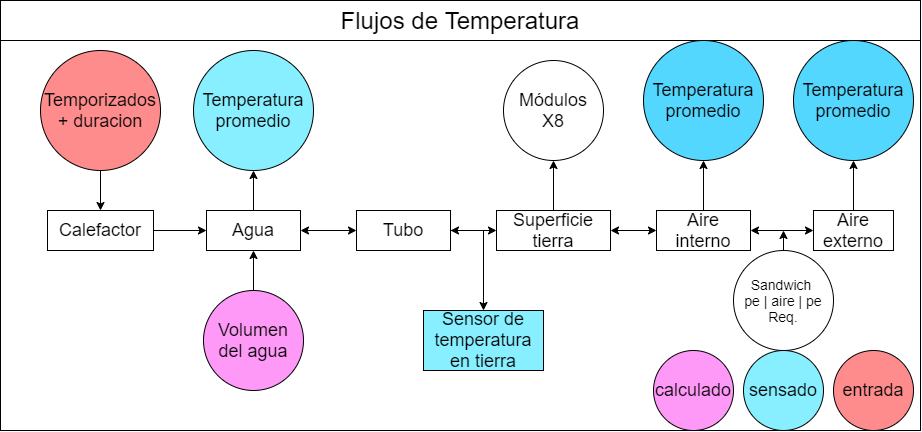
\includegraphics[width=.85\linewidth]{imagenes/flujos de calor.png} 
%				\caption{Relación entre sistemas desarrollados}
%				\label{fig:flujo_calor}
%			\end{figure}

%		\end{itemize}

\subsection{Modelo de optimización}
	
		
	\subsubsection{Descripción del problema}
			
	Se cuenta con un invernadero, el cual requiere de distintos costos. Uno de estos viene dado por el funcionamiento del calefactor junto a la bomba de calefacción $BT$, más el funcionamiento de la bomba de irrigación $BA$ por sus costos respectivos de electricidad $ce$, más el costo del agua $ca$ utilizada para la irrigación.
	
	Por otro lado, es necesario mantener un rango para la temperatura de agua entre $ta_{min}$ y $ta_{max}$; la temperatura del suelo entre $tp_{min}$ y  $tp_{max}$; y la humedad relativa del suelo entre $hs_{min}$ y $hs_{max}$.
				

				Cada temperatura en el tiempo se calculará según la ecuación \ref{eq:delta_t}.
				
				
				
				\begin{equation} 
				\Delta T = \frac{\Delta \dot{Q} * p}{Cm * m}
				\label{eq:delta_t}
				\end{equation}
				
	Donde $\Delta \dot{Q}$ representa la transferencia de calor neta, $p$ representa el periodo entre cada tiempo (en segundos), $Cm$ representa el calor específico del material y $m$ representa la masa del material involucrado en la transferencia de calor. Además, cada flujo de calor, a excepción del generado por el calefactor, puede ser calculando según la ecuación \ref{eq:delta_q} donde la $R$ corresponde a la resistencia térmica y $T$ es la temperatura.
				
				
				
				\begin{equation}
				 \dot{Q} = \frac{T_{1}-T_{2}}{R}
				\label{eq:delta_q}
				\end{equation}
				
				
				
				Finalmente, la humedad relativa es calculada por la ecuación \ref{eq:delta_h}, donde $Fe$ es la función que caracteriza la disminución de la humedad relativa en el tiempo y $Aa$ es el porcentaje en que aumenta la humedad relativa cuando se activa la bomba de irrigación $BA$	.
				
				\begin{equation}
				\Delta H \, = \, Fe*BA_{t}\,+\, Aa*(BA_{t}-1)
				\label{eq:delta_h}
				\end{equation}

	

	\subsection{Sistema de gestión}
		
	La realización de la automatización de esta investigación necesita un protocolo de transporte de mensajes, el cual facilite la comunicación entre múltiples dispositivos por que utilizara el protocolo MQTT. Además, se necesita emplear una base de datos para almacenar los datos que vaya controlando el invernadero. 
	
	Dado que no existe un transpaso directo entre el protocolo de transporte y la base de datos, en los resultados se implementará una cara para cumplir dicha acción mediante un analizador sintáctico o ''parsers''. De igual manera, para comunicar el invernadero con el modelo de optimización se requiere otra aplicación capaz de adquirir los valores actuales de la base da datos, ejecutar el modelo y enviar el control óptimo resultante. En la figura \ref{fig:sist_gest} se muestra un esquema del sistema de gestión resultante, el muestra cómo se relacionan estos elementos
	
	\begin{figure}[h!]
	\centering
 	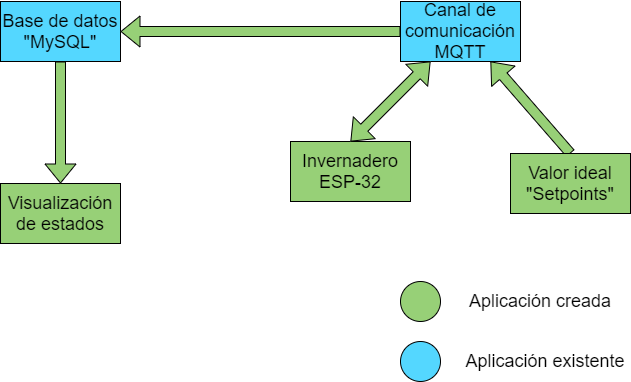
\includegraphics[width=0.8	\linewidth]{imagenes/sistema de gestion .png}
	\caption{Sistema de gestión}
	\label{fig:sist_gest}
	\end{figure}

	% Todo esto es parte de tus resultados, ojo ahí!!!
%		\subsubsection{Parser MQTT $ \rightarrow $ SQL}
%			\label{parser}
%			Debido a  los múltiples tipos de mensajes que pueden ser transmitidos dentro de los tópicos del MQTT, se optó por codificar los mensajes en formato "JSON" (Javascript object notation) por su simpleza en el orden del contenido de los mensajes. Los mensajes se encuentran descritos en la Figura \ref{fig:mensajes}.
%			
%			\begin{figure}[ht]
%				\centering
%				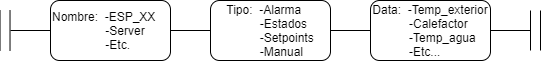
\includegraphics[width=.85\linewidth]{imagenes/mensajes.png} 
%				\caption{Formato de los mensajes dentro del MQTT}
%				\label{fig:mensajes}
%			\end{figure}
%			
%			Ya que los mensajes solo estarán disponibles dentro de los tópicos del MQTT, se realizó una aplicación en Java que realice lo siguiente:
%			\begin{itemize}
%				\item Conectarse a los tópicos relevantes (entradas y salidas).
%				\item Procesar el mensaje en JSON a formato SQL.
%				\item Conectarse a la base de datos MySQL.
%				\item Enviar el mensaje procesado o notificar si hubo un error.
%			\end{itemize}
%			
%	
%		\subsubsection{Comunicación modelo $\rightarrow$ invernadero}
%			Dado que el control del invernadero propuesto es determinado por un modelo de optimización para las variables de irrigación y temperatura, se desarrolló un programa capaz de ejecutar dicho modelo, tomando como entrada el estado actual del invernadero y reenviando al invernadero el control optimo según la respuesta del modelo.


				
\newpage
\section{Bibliografía}

\printbibliography


\end{document}
